\documentclass[14pt]{extarticle}
\usepackage{fontspec}
\usepackage{polyglossia}
\usepackage{amsmath}
\usepackage{amssymb}
\usepackage{xcolor}
\usepackage{fancyhdr}
\usepackage{graphicx}
\usepackage{listings}
\usepackage[most]{tcolorbox}
% \usepackage{setspace}
\usepackage{pifont}
\usepackage{enumitem}
\usepackage{titlesec}
\usepackage[bottom]{footmisc}
\usepackage{titling}
\usepackage{minted}
\usepackage{etoolbox}
\usepackage{array}
\usepackage{longtable} % page-breakable tables (must load before polyglossia/bidi RTL setup)
\usepackage{extsizes}
\usepackage{float}
\usepackage{booktabs}
\usepackage{hyperref}
\usepackage[onehalfspacing]{setspace}
\newif\ifwhiteblack
\ifdefined\setwhiteblack
  \setwhiteblack
\fi

\ifwhiteblack
  \usepackage[a4paper, landscape, top=1.25cm, bottom=1.25cm, left=1.25cm, right=1.25cm, headheight=1.5cm, headsep=0.5cm]{geometry}
\else
  \usepackage[a4paper, top=2.7cm, bottom=2.7cm, left=2.5cm, right=2.5cm, headheight=1.5cm, headsep=0.5cm]{geometry}
\fi
\usepackage{tikz}
\usepackage{datetime2}

\usetikzlibrary{automata, positioning, arrows.meta, arrows}
\providecommand{\LTcaptype}{table}

\newfontfamily\emoji{Segoe UI Emoji}

\pagestyle{fancy}

\setmainlanguage[numerals=western]{arabic}
\setotherlanguage{english}
\newfontfamily\arabicfont[Script=Arabic]{Calibri}
\newfontfamily\arabicfonttt[Script=Arabic]{Courier New}



\ifwhiteblack
\lstset{
  language=[Sharp]C,
  numbers=left,
  stepnumber=1,
  numbersep=8pt,
  frame=single,
  basicstyle=\ttfamily\small,
  keywordstyle=\bfseries,
  stringstyle=\ttfamily,
  commentstyle=\itshape
}
\else
\lstset{
  language=[Sharp]C,
  numbers=left,
  stepnumber=1,
  numbersep=8pt,
  frame=single,
  basicstyle=\ttfamily\small,
  keywordstyle=\color{blue},
  stringstyle=\color{red},
  commentstyle=\color{green!50!black}
}
\fi

\newif\ifdetailed
\ifdefined\setdetailed
  \setdetailed
\fi

\newif\ifwithsols
\ifdefined\setwithsols
  \setwithsols
\fi

\ifwhiteblack
  \AtBeginDocument{
    \LARGE
    \usemintedstyle{bw}
  }
\fi

% Default minted look: compact code that wraps long lines.
% Not applied in black-and-white landscape mode, which already uses \LARGE.
\ifwhiteblack\else
  \setminted{fontsize=\small, breaklines=true}
\fi

% unified tcolorboxes for articles
\ifwhiteblack
\tcbset{colback=white, colframe=black, fonttitle=\bfseries, boxrule=1pt}
\newtcolorbox{boxDef}[1][]{title={{\emoji📘} تعريف\ifx\\#1\\\else ~#1\fi :}}
\newtcolorbox{boxExercise}[1][]{title={{\emoji🧩} تمرين\ifx\\#1\\\else ~#1\fi :}}
\newtcolorbox{boxExample}[1][]{title={{\emoji📝} مثال\ifx\\#1\\\else ~#1\fi :}}
\newtcolorbox{boxNote}[1][]{title={{\emoji✨} ملاحظة\ifx\\#1\\\else ~#1\fi :}}
\newtcolorbox{boxAttention}[1][]{title={{\emoji🔔} تنبيه\ifx\\#1\\\else ~#1\fi :}}
\newtcolorbox{boxWarning}[1][]{title={{\emoji⚡} ملاحظة هامة\ifx\\#1\\\else ~#1\fi :}}
\newtcolorbox{boxSolution}[1][]{title={{\emoji✅} حل\ifx\\#1\\\else ~#1\fi :}}
\newtcolorbox{boxSymbol}[1][]{title={{\emoji🔣} رمز\ifx\\#1\\\else ~#1\fi :}}
\newtcolorbox{boxHint}[1][]{title={{\emoji💡} تلميح\ifx\\#1\\\else ~#1\fi :}}
\else
\tcbset{colback=white, colframe=black, fonttitle=\bfseries, boxrule=0.8pt}
\newtcolorbox{boxDef}[1][]{colback=blue!5!white,colframe=blue!75!black,
  title={{\emoji📘} تعريف\ifx\\#1\\\else ~#1\fi :}}
\newtcolorbox{boxExercise}[1][]{colback=cyan!5!white,colframe=cyan!70!black,
  title={{\emoji🧩} تمرين\ifx\\#1\\\else ~#1\fi :}}
\newtcolorbox{boxExample}[1][]{colback=yellow!5!white,colframe=orange!90!black,
  title={{\emoji📝} مثال\ifx\\#1\\\else ~#1\fi :}}
\newtcolorbox{boxNote}[1][]{colback=gray!10!white,colframe=black,
  title={{\emoji✨} ملاحظة\ifx\\#1\\\else ~#1\fi :}}
\newtcolorbox{boxAttention}[1][]{colback=magenta!10!white,colframe=magenta!80!black,
  title={{\emoji🔔} تنبيه\ifx\\#1\\\else ~#1\fi :}}
\newtcolorbox{boxWarning}[1][]{colback=red!5!white,colframe=red!75!black,
  title={{\emoji⚡} ملاحظة هامة\ifx\\#1\\\else ~#1\fi :}}
\newtcolorbox{boxSolution}[1][]{colback=green!5!white,colframe=green!60!black,
  title={{\emoji✅} حل\ifx\\#1\\\else ~#1\fi :}}
\newtcolorbox{boxSymbol}[1][]{colback=purple!5!white,colframe=purple!70!black,
  title={{\emoji🔣} رمز\ifx\\#1\\\else ~#1\fi :}}
\newtcolorbox{boxHint}[1][]{colback=teal!5!white,colframe=teal!60!black,
  title={{\emoji💡} تلميح\ifx\\#1\\\else ~#1\fi :}}
\fi


\ifwhiteblack
\tcbset{simplecode/.style={ colback=white, colframe=black, boxrule=1pt, arc=2pt, left=4pt,right=4pt,top=4pt,bottom=4pt}}
\else
\tcbset{simplecode/.style={ colback=gray!5, colframe=black!50, boxrule=0.4pt, arc=2pt, left=4pt,right=4pt,top=4pt,bottom=4pt}}
\fi
% Compact code boxes: tighter line spacing (the preamble uses onehalfspacing) and small vertical gaps.
% Must come AFTER the simplecode definition above.
\tcbset{simplecode/.append style={fontupper=\setstretch{0.95}, top=4pt, bottom=4pt, before skip=6pt, after skip=6pt}}
\newenvironment{boxCode}{\begin{tcolorbox}[simplecode]}{\end{tcolorbox}}

% Code cell used inside tables (keeps code left-to-right inside RTL tables).
% Use inside a fixed-width p{...} column: \begin{pycell}\begin{minted}...\end{minted}\end{pycell}
\newtcolorbox{pycell}{frame empty,colback=white,boxsep=0pt,left=2pt,right=2pt,top=2pt,bottom=2pt,width=\linewidth}

\newcolumntype{C}[1]{>{\centering\arraybackslash}p{#1}}

\makeatletter
\DTMnewdatestyle{dotted}{%
  \renewcommand{\DTMdisplaydate}[4]{\two@digits{##3}.\two@digits{##2}.##1}%
  \renewcommand{\DTMDisplaydate}{\DTMdisplaydate}%
}
\makeatother
\DTMsetdatestyle{dotted}

% redefine spaces after titles
\makeatletter
\renewcommand{\@maketitle}{%
  \begin{center}
    {\huge \bfseries \@title \par}%
    \vskip 0.2em % space between title and author
    {\large \@author \par}%
    % \vskip 0.2em % space between author and date
    % {\normalsize \@date \par}%
    {\small \hfill \begin{english}\DTMtoday\end{english} \par}%
  \end{center}
}
\makeatother

\fancyhf{} % clear default
\fancypagestyle{plain}{
  \fancyhf{}
  \fancyhead[L]{مدرسة التسامح الشاملة}
  % \fancyhead[L]{
\includegraphics[height=1cm]{../../../images/logoTasamoh.png}}
  \fancyhead[R]{الأستاذ محمود اغبارية}
  \fancyfoot[C]{\thepage}
}

\fancyhead[L]{مدرسة التسامح الشاملة}
\fancyhead[R]{الأستاذ محمود اغبارية}
\fancyfoot[C]{\thepage}

\setcounter{tocdepth}{3} % only section subsection and subsubsection in TOC

\newcommand{\importpdfpage}[2]{%
    \thispagestyle{empty}
    \newgeometry{left=0cm,right=0cm,top=0cm,bottom=0cm}
    \includegraphics[page=#2,width=0.95\paperwidth,height=0.95\paperheight,keepaspectratio]{#1}
    \restoregeometry
}

\newcommand{\insertFullImg}[1]{%
    \noindent
    \makebox[\textwidth][c]{
        \includegraphics[width=0.9\paperwidth,keepaspectratio]{#1}%
    }%
}%


\ifwithsols
\title{حل ورقة تمرن $10$ للصف العاشر $10$ - أسئلة عامة وأسئلة بجروت في الحلقات}
\else
\title{ورقة تمرن $10$ للصف العاشر $10$ - أسئلة عامة وأسئلة بجروت في الحلقات}
\fi

\begin{document}

\maketitle
\thispagestyle{fancy}

% ==============================================================
% القسم الأول: أسئلة عامة عن الحلقات
% ==============================================================
\section*{القسم الأوّل: أسئلة عامة في الحلقات}

\begin{enumerate}[itemsep=2em]

% --- أ: البحث عن قوى وأقرب قيمة لهدف ---
\item اكتب عملية خارجية تتلقى عددًا صحيحًا موجبًا $x$. \\
على العملية أن تجد وتعيد أصغر عدد يكون من قوى العدد $2$ ولكنه أكبر تمامًا من $x$. \\
\textbf{مثال:} إذا كان المعطى $10$، تُعيد العملية $16$. وإذا كان المعطى $50$، تُعيد $64$.
\ifwithsols
\begin{boxSolution}
\begin{english}
\begin{minted}{csharp}
public static int NextPowerOf2(int x)
{
    int p = 1;
    while (p <= x)
    {
        p *= 2;
    }
    return p;
}
\end{minted}
\end{english}
\end{boxSolution}
\fi
\filbreak

\item اكتب برنامجًا يستقبل عددًا صحيحًا يمثّل هدفًا (\textenglish{target})، ثم يستقبل $20$ عددًا صحيحًا، وفي النهاية يطبع العدد الأقرب إلى \textenglish{target} من بين الأعداد الـ $20$ (أي العدد الذي تكون القيمة المطلقة للفرق بينه وبين \textenglish{target} هي الأصغر). \\
\textbf{مثال:} إذا كان الهدف $50$ ومن بين الأعداد المدخلة ظهر $47$ و $55$، فإنّ $47$ أقرب إلى $50$ لأنّ $|47 - 50| = 3$ بينما $|55 - 50| = 5$.
\ifwithsols
\begin{boxSolution}
\begin{english}
\begin{minted}{csharp}
int target = int.Parse(Console.ReadLine());
int closest = int.Parse(Console.ReadLine());
int minDiff = Math.Abs(closest - target);

for (int i = 1; i < 20; i++)
{
    int x = int.Parse(Console.ReadLine());
    int diff = Math.Abs(x - target);
    if (diff < minDiff)
    {
        minDiff = diff;
        closest = x;
    }
}
Console.WriteLine("Closest number = " + closest);
\end{minted}
\end{english}
\end{boxSolution}
\fi
\filbreak

% --- ب: مقارنة أعداد متتالية (نافذة متحركة من عنصرين أو ثلاثة) ---
\item اكتب برنامجًا يستقبل $20$ عددًا صحيحًا ويطبع مجموع كل عددين متتاليين. \\
أي إذا كانت المدخلات: $a_1, a_2, a_3, \ldots$ فعليه أن يطبع: $(a_1 + a_2), (a_2 + a_3), \ldots$
\ifwithsols
\begin{boxSolution}
\begin{english}
\begin{minted}{csharp}
int prev = int.Parse(Console.ReadLine());
for (int i = 1; i < 20; i++)
{
    int x = int.Parse(Console.ReadLine());
    Console.WriteLine(prev + x);
    prev = x;
}
\end{minted}
\end{english}
\end{boxSolution}
\fi
\filbreak

\item اكتب برنامجًا يستقبل من المستخدم $15$ عددًا صحيحًا ويطبع عدد الأعداد التي تقبل القسمة على العدد الذي قبلها مباشرة بدون باقٍ.
\ifdetailed
\begin{boxExample}
إذا أدخل المستخدم الأعداد: $4, 12, 5, 10$:
\begin{itemize}[nosep]
    \item العدد $12$ يقبل القسمة على $4$ $\leftarrow$ نعدّه.
    \item العدد $5$ لا يقبل القسمة على $12$.
    \item العدد $10$ يقبل القسمة على $5$ $\leftarrow$ نعدّه.
\end{itemize}
النتيجة: $2$.
\end{boxExample}
\fi
\ifwithsols
\begin{boxSolution}
\begin{english}
\begin{minted}{csharp}
int prev = int.Parse(Console.ReadLine());
int cnt = 0;

for (int i = 1; i < 15; i++)
{
    int x = int.Parse(Console.ReadLine());
    if (prev != 0 && x % prev == 0)
    {
        cnt++;
    }
    prev = x;
}
Console.WriteLine(cnt);
\end{minted}
\end{english}
\end{boxSolution}
\fi
\filbreak

\item اكتب برنامجًا يستقبل من المستخدم $20$ عددًا صحيحًا غير صفري (موجبة أو سالبة)، ويطبع عدد المرّات التي تغيّرت فيها الإشارة بين عددين متتاليين (من موجب إلى سالب أو من سالب إلى موجب). \\
\textbf{مثال:} في السلسلة $4, 7, -2, -5, 3, -1$ تغيّرت الإشارة $3$ مرّات (بين $7$ و $-2$، وبين $-5$ و $3$، وبين $3$ و $-1$).
\ifwithsols
\begin{boxSolution}
\begin{english}
\begin{minted}{csharp}
int prev = int.Parse(Console.ReadLine());
int signChanges = 0;

for (int i = 1; i < 20; i++)
{
    int x = int.Parse(Console.ReadLine());
    if ((prev > 0 && x < 0) || (prev < 0 && x > 0))
    {
        signChanges++;
    }
    prev = x;
}
Console.WriteLine(signChanges);
\end{minted}
\end{english}
\end{boxSolution}
\fi
\filbreak

\item اكتب برنامجًا يستقبل $25$ عددًا صحيحًا ويطبع عدد الأعداد التي تساوي مجموع العددين اللذين سبقاها مباشرة (أي: $x_i = x_{i-1} + x_{i-2}$).
\ifdetailed
\begin{boxExample}
المدخلات: $1, 4, 5, 20, 25, \ldots$
\begin{itemize}[nosep]
    \item العدد $5$ يساوي $1 + 4$ $\leftarrow$ نعدّه.
    \item العدد $25$ يساوي $5 + 20$ $\leftarrow$ نعدّه.
\end{itemize}
\end{boxExample}
\fi
\ifwithsols
\begin{boxSolution}
\begin{english}
\begin{minted}{csharp}
int a = int.Parse(Console.ReadLine());
int b = int.Parse(Console.ReadLine());
int cnt = 0;

for (int i = 2; i < 25; i++)
{
    int x = int.Parse(Console.ReadLine());
    if (x == a + b)
    {
        cnt++;
    }
    a = b;
    b = x;
}
Console.WriteLine(cnt);
\end{minted}
\end{english}
\end{boxSolution}
\fi
\filbreak

% --- ج: فحص خصائص سلسلة كاملة وطول أطول سلسلة متتالية (Streaks) ---
\item اكتب برنامجًا يستقبل $15$ عددًا صحيحًا، ويفحص هل جميع الأعداد المدخلة مرتّبة بترتيب تصاعدي تمامًا (أي أنّ كل عدد أكبر تمامًا من العدد الذي سبقه). \\
في النهاية يطبع البرنامج \textenglish{"Ascending"} إذا كانت السلسلة كلّها تصاعدية، و \textenglish{"Not Ascending"} خلاف ذلك.
\ifwithsols
\begin{boxSolution}
\begin{english}
\begin{minted}{csharp}
int prev = int.Parse(Console.ReadLine());
bool isAscending = true;

for (int i = 1; i < 15; i++)
{
    int x = int.Parse(Console.ReadLine());
    if (x <= prev)
    {
        isAscending = false;
    }
    prev = x;
}

if (isAscending)
{
    Console.WriteLine("Ascending");
}
else
{
    Console.WriteLine("Not Ascending");
}
\end{minted}
\end{english}
\end{boxSolution}
\fi
\filbreak

\item اكتب برنامجًا يستقبل $12$ عددًا صحيحًا ويفحص هل ظهر العدد $5$ ثلاث مرّات متتالية على الأقل. \\
في النهاية يطبع البرنامج \textenglish{"Yes"} إذا ظهر ثلاث مرّات متتالية، و \textenglish{"No"} وإلا.
\ifwithsols
\begin{boxSolution}
\begin{english}
\begin{minted}{csharp}
int cnt = 0;
bool ok = false;

for (int i = 0; i < 12; i++)
{
    int x = int.Parse(Console.ReadLine());
    if (x == 5)
    {
        cnt++;
        if (cnt == 3)
        {
            ok = true;
        }
    }
    else
    {
        cnt = 0;
    }
}

if (ok)
{
    Console.WriteLine("Yes");
}
else
{
    Console.WriteLine("No");
}
\end{minted}
\end{english}
\end{boxSolution}
\fi
\filbreak

\item اكتب برنامجًا يستقبل $30$ عددًا صحيحًا ويطبع طول أطول سلسلة متتالية من الأعداد السالبة.
\ifwithsols
\begin{boxSolution}
\begin{english}
\begin{minted}{csharp}
int maxSeq = 0, curr = 0;

for (int i = 0; i < 30; i++)
{
    int x = int.Parse(Console.ReadLine());
    if (x < 0)
    {
        curr++;
        if (curr > maxSeq)
        {
            maxSeq = curr;
        }
    }
    else
    {
        curr = 0;
    }
}
Console.WriteLine(maxSeq);
\end{minted}
\end{english}
\end{boxSolution}
\fi
\filbreak

\item اكتب برنامجًا يستقبل $15$ عددًا صحيحًا ويطبع طول أطول سلسلة تصاعدية متتالية (السلسلة التصاعدية هي التي يكون فيها كل عدد أكبر تمامًا من العدد الذي سبقه مباشرة).
\ifwithsols
\begin{boxSolution}
\begin{english}
\begin{minted}{csharp}
int prev = int.Parse(Console.ReadLine());
int currLen = 1, maxLen = 1;

for (int i = 1; i < 15; i++)
{
    int x = int.Parse(Console.ReadLine());
    if (x > prev)
    {
        currLen++;
    }
    else
    {
        currLen = 1;
    }

    if (currLen > maxLen)
    {
        maxLen = currLen;
    }
    prev = x;
}
Console.WriteLine(maxLen);
\end{minted}
\end{english}
\end{boxSolution}
\fi
\filbreak

\end{enumerate}

\clearpage
% ==============================================================
% القسم الثاني: أسئلة بجروت عن الحلقات
% ==============================================================
\section*{القسم الثاني: أسئلة بجروت في الحلقات}

\subsection*{سؤال 5 امتحان 899222 سنة 2011}
\addcontentsline{toc}{subsection}{سؤال 5 امتحان 899222 سنة 2011}

\insertFullImg{../../../bagrut_questions/basics/loops_for_2011_899222_5.png}

\ifwithsols
\begin{boxSolution}[سؤال 5 امتحان 899222 سنة 2011]
\begin{boxCode}
\begin{english}
\begin{minted}{csharp}
int num1 = int.Parse(Console.ReadLine());
int num2 = int.Parse(Console.ReadLine());
int previousSum = num1 + num2;

for (int i = 2; i <= 218; i++)
{
    int currentNum1 = int.Parse(Console.ReadLine());
    int currentNum2 = int.Parse(Console.ReadLine());
    int currentSum = currentNum1 + currentNum2;

    if (currentSum < previousSum)
        Console.WriteLine("smaller");

    previousSum = currentSum;
}
\end{minted}
\end{english}
\end{boxCode}
\end{boxSolution}
\fi


\subsection*{سؤال 6 امتحان 899222 سنة 2013}

\importpdfpage{../../../bagrut_questions/basics/loops_for_2013_899222_6.pdf}{1}

\ifwithsols
\subsubsection*{حل سؤال 6 امتحان 899222 سنة 2013}:
\bigskip
% // TODO:
\fi


\importpdfpage{../../../bagrut_questions/basics/loops_for_2013_899222_10.pdf}{1}

\ifwithsols

\paragraph*{حل سؤال 10 امتحان 899222 سنة 2013}:
\bigskip

% // TODO:

\fi


\subsection*{سؤال 2 امتحان 899371 سنة 2023}

\insertFullImg{../../../bagrut_questions/basics/loops_for_2023_899371_2.png}

\ifwithsols
\begin{boxSolution}[سؤال 2 امتحان 899371 سنة 2023]
\begin{enumerate}[itemsep=1.5em, label=\alph*.]
    \item // TODO:
\end{enumerate}
\end{boxSolution}
\clearpage
\fi


\subsection*{سؤال 7 امتحان 899222 سنة 2015}
\addcontentsline{toc}{subsection}{سؤال 7 امتحان 899222 سنة 2015}

\noindent
    \makebox[\textwidth][c]{
        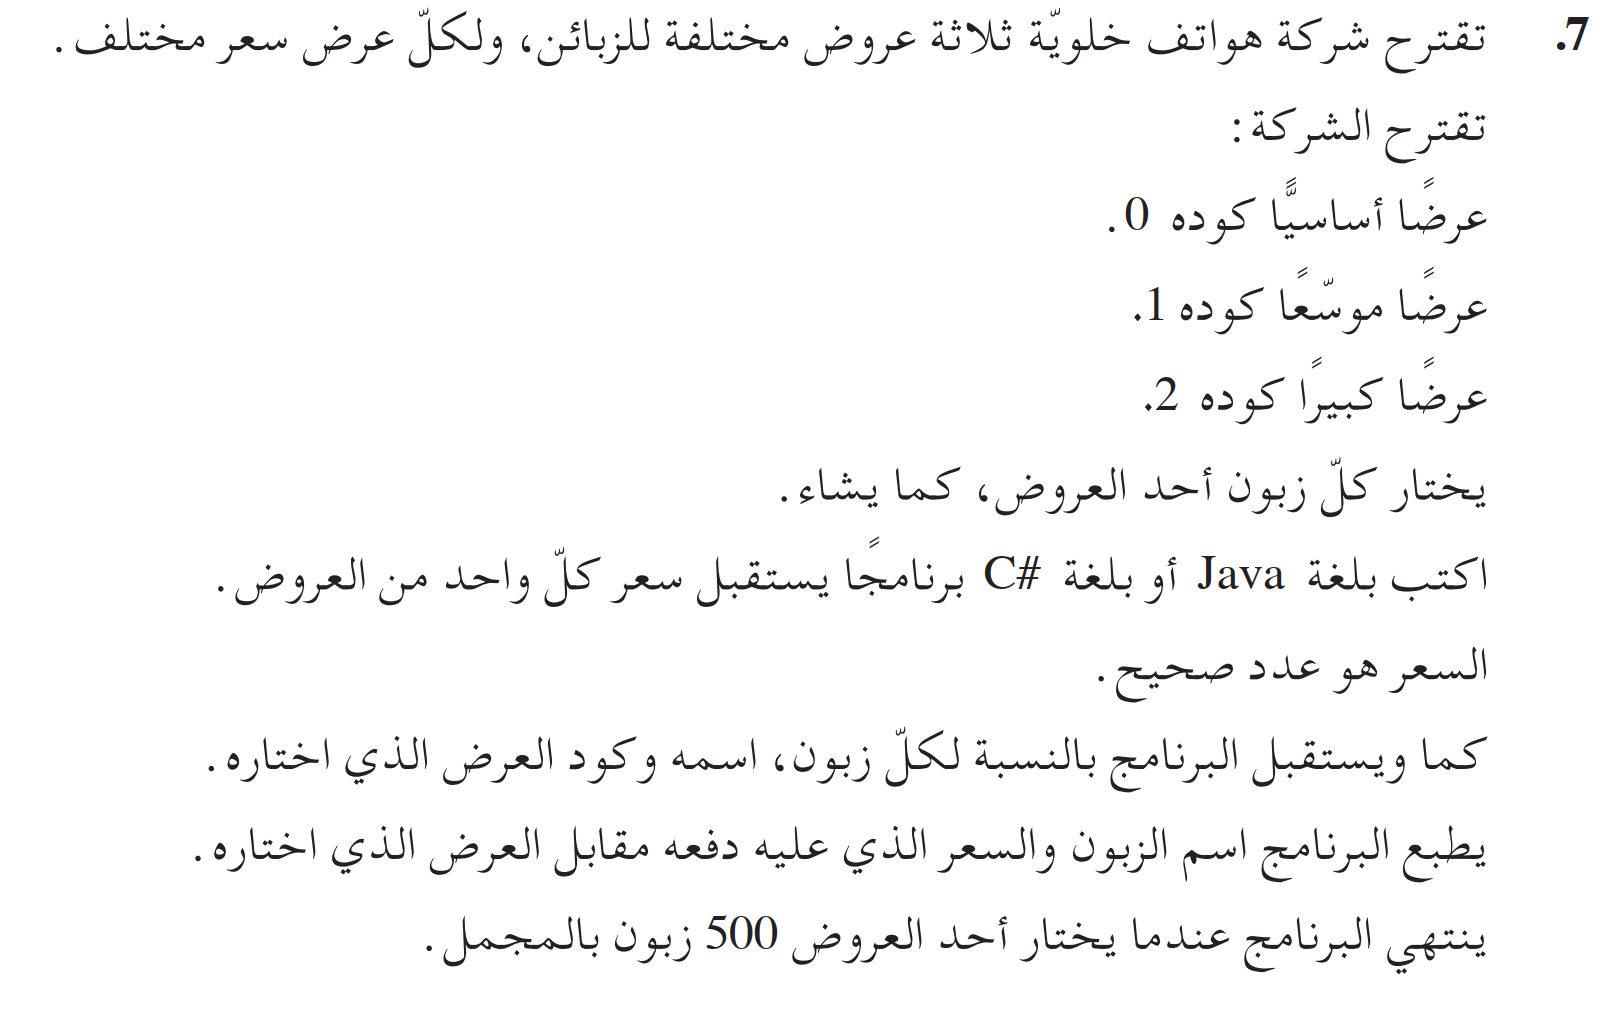
\includegraphics[width=0.9\paperwidth,keepaspectratio]{ ../../../bagrut_questions/basics/loops_while_2015_899222_7.png }%
    }%

\ifwithsols
\begin{boxSolution}[سؤال 7 امتحان 899222 سنة 2015]
\begin{boxCode}
\begin{english}
\begin{minted}{csharp}
int price0 = int.Parse(Console.ReadLine());
int price1 = int.Parse(Console.ReadLine());
int price2 = int.Parse(Console.ReadLine());
int cnt0 = 0, cnt1 = 0, cnt2 = 0;

while (cnt0 < 500 && cnt1 < 500 && cnt2 < 500)
{
    string name = Console.ReadLine();
    int offerCode = int.Parse(Console.ReadLine());

    Console.WriteLine("Customer Name: " + name);
    if (offerCode == 0)
    {
        Console.WriteLine("Price: " + price0);
        cnt0++;
    }
    else if (offerCode == 1)
    {
        Console.WriteLine("Price: " + price1);
        cnt1++;
    }
    else if (offerCode == 2)
    {
        Console.WriteLine("Price: " + price2);
        cnt2++;
    }
}
\end{minted}
\end{english}
\end{boxCode}

\end{boxSolution}
\clearpage
\fi


\subsection*{سؤال 8 امتحان 899222 سنة 2013}

\importpdfpage{../../../bagrut_questions/basics/loops_while_2013_899222_8.pdf}{1}

\ifwithsols
\subsubsection*{حل سؤال 8 امتحان 899222 سنة 2013}:
\bigskip
% // TODO:
\fi


\vspace{1cm}
\begin{flushleft}
أرجو لكم وقتًا ممتعًا.

الأستاذ محمود اغبارية.
\end{flushleft}

\end{document}
